\documentclass[letterpaper,12pt,twoside,]{pinp}

%% Some pieces required from the pandoc template
\providecommand{\tightlist}{%
  \setlength{\itemsep}{0pt}\setlength{\parskip}{0pt}}

% Use the lineno option to display guide line numbers if required.
% Note that the use of elements such as single-column equations
% may affect the guide line number alignment.

\usepackage[T1]{fontenc}
\usepackage[utf8]{inputenc}

% pinp change: the geometry package layout settings need to be set here, not in pinp.cls
\geometry{layoutsize={0.95588\paperwidth,0.98864\paperheight},%
  layouthoffset=0.02206\paperwidth, layoutvoffset=0.00568\paperheight}

\definecolor{pinpblue}{HTML}{185FAF}  % imagecolorpicker on blue for new R logo
\definecolor{pnasbluetext}{RGB}{101,0,0} %



\title{Lab 001-1 - Getting Started with R and RStudio}

\author[a]{EPIB607 - Inferential Statistics}

  \affil[a]{Fall 2020, McGill University}

\setcounter{secnumdepth}{5}

% Please give the surname of the lead author for the running footer
\leadauthor{}

% Keywords are not mandatory, but authors are strongly encouraged to provide them. If provided, please include two to five keywords, separated by the pipe symbol, e.g:
 \keywords{  R |  RStudio  }  

\begin{abstract}

\end{abstract}

\dates{This version was compiled on \today} 

% initially we use doi so keep for backwards compatibility
% new name is doi_footer

\pinpfootercontents{Lab 001-1}

\begin{document}

% Optional adjustment to line up main text (after abstract) of first page with line numbers, when using both lineno and twocolumn options.
% You should only change this length when you've finalised the article contents.
\verticaladjustment{-2pt}

\maketitle
\thispagestyle{firststyle}
\ifthenelse{\boolean{shortarticle}}{\ifthenelse{\boolean{singlecolumn}}{\abscontentformatted}{\abscontent}}{}

% If your first paragraph (i.e. with the \dropcap) contains a list environment (quote, quotation, theorem, definition, enumerate, itemize...), the line after the list may have some extra indentation. If this is the case, add \parshape=0 to the end of the list environment.


\tableofcontents

\textsf{R} is an open-source statistical language widely used in
biostatistics and computational biology, among other fields of research.
\textit{RStudio} is a ``front end'' to \textsf{R} that simplifies
important aspects of using \textsf{R} and makes it much easier to work
within the \textsf{R} environment. Both \textsf{R} and \textit{RStudio}
run identically under the Mac OSX, Microsoft Windows, and Linux.

\hypertarget{installing-and}{%
\section{\texorpdfstring{Installing \textsf{R} and
\textit{RStudio}}{Installing  and }}\label{installing-and}}

First, download \textsf{R} from \url{http://cran.us.r-project.org/}.
Versions are available for Windows, Mac OS X, and Linux. Follow the
instructions when running the installation program, selecting the
default options when prompted.

\textit{RStudio} can be downloaded from
\url{https://www.rstudio.com/products/rstudio/download/}. Scroll down to
``Installers for Supported Platforms'' and select the appropriate
version for your system. Leave all default settings in the installation
options.

\hypertarget{the-rstudio-console}{%
\section{The RStudio Console}\label{the-rstudio-console}}

\centerline{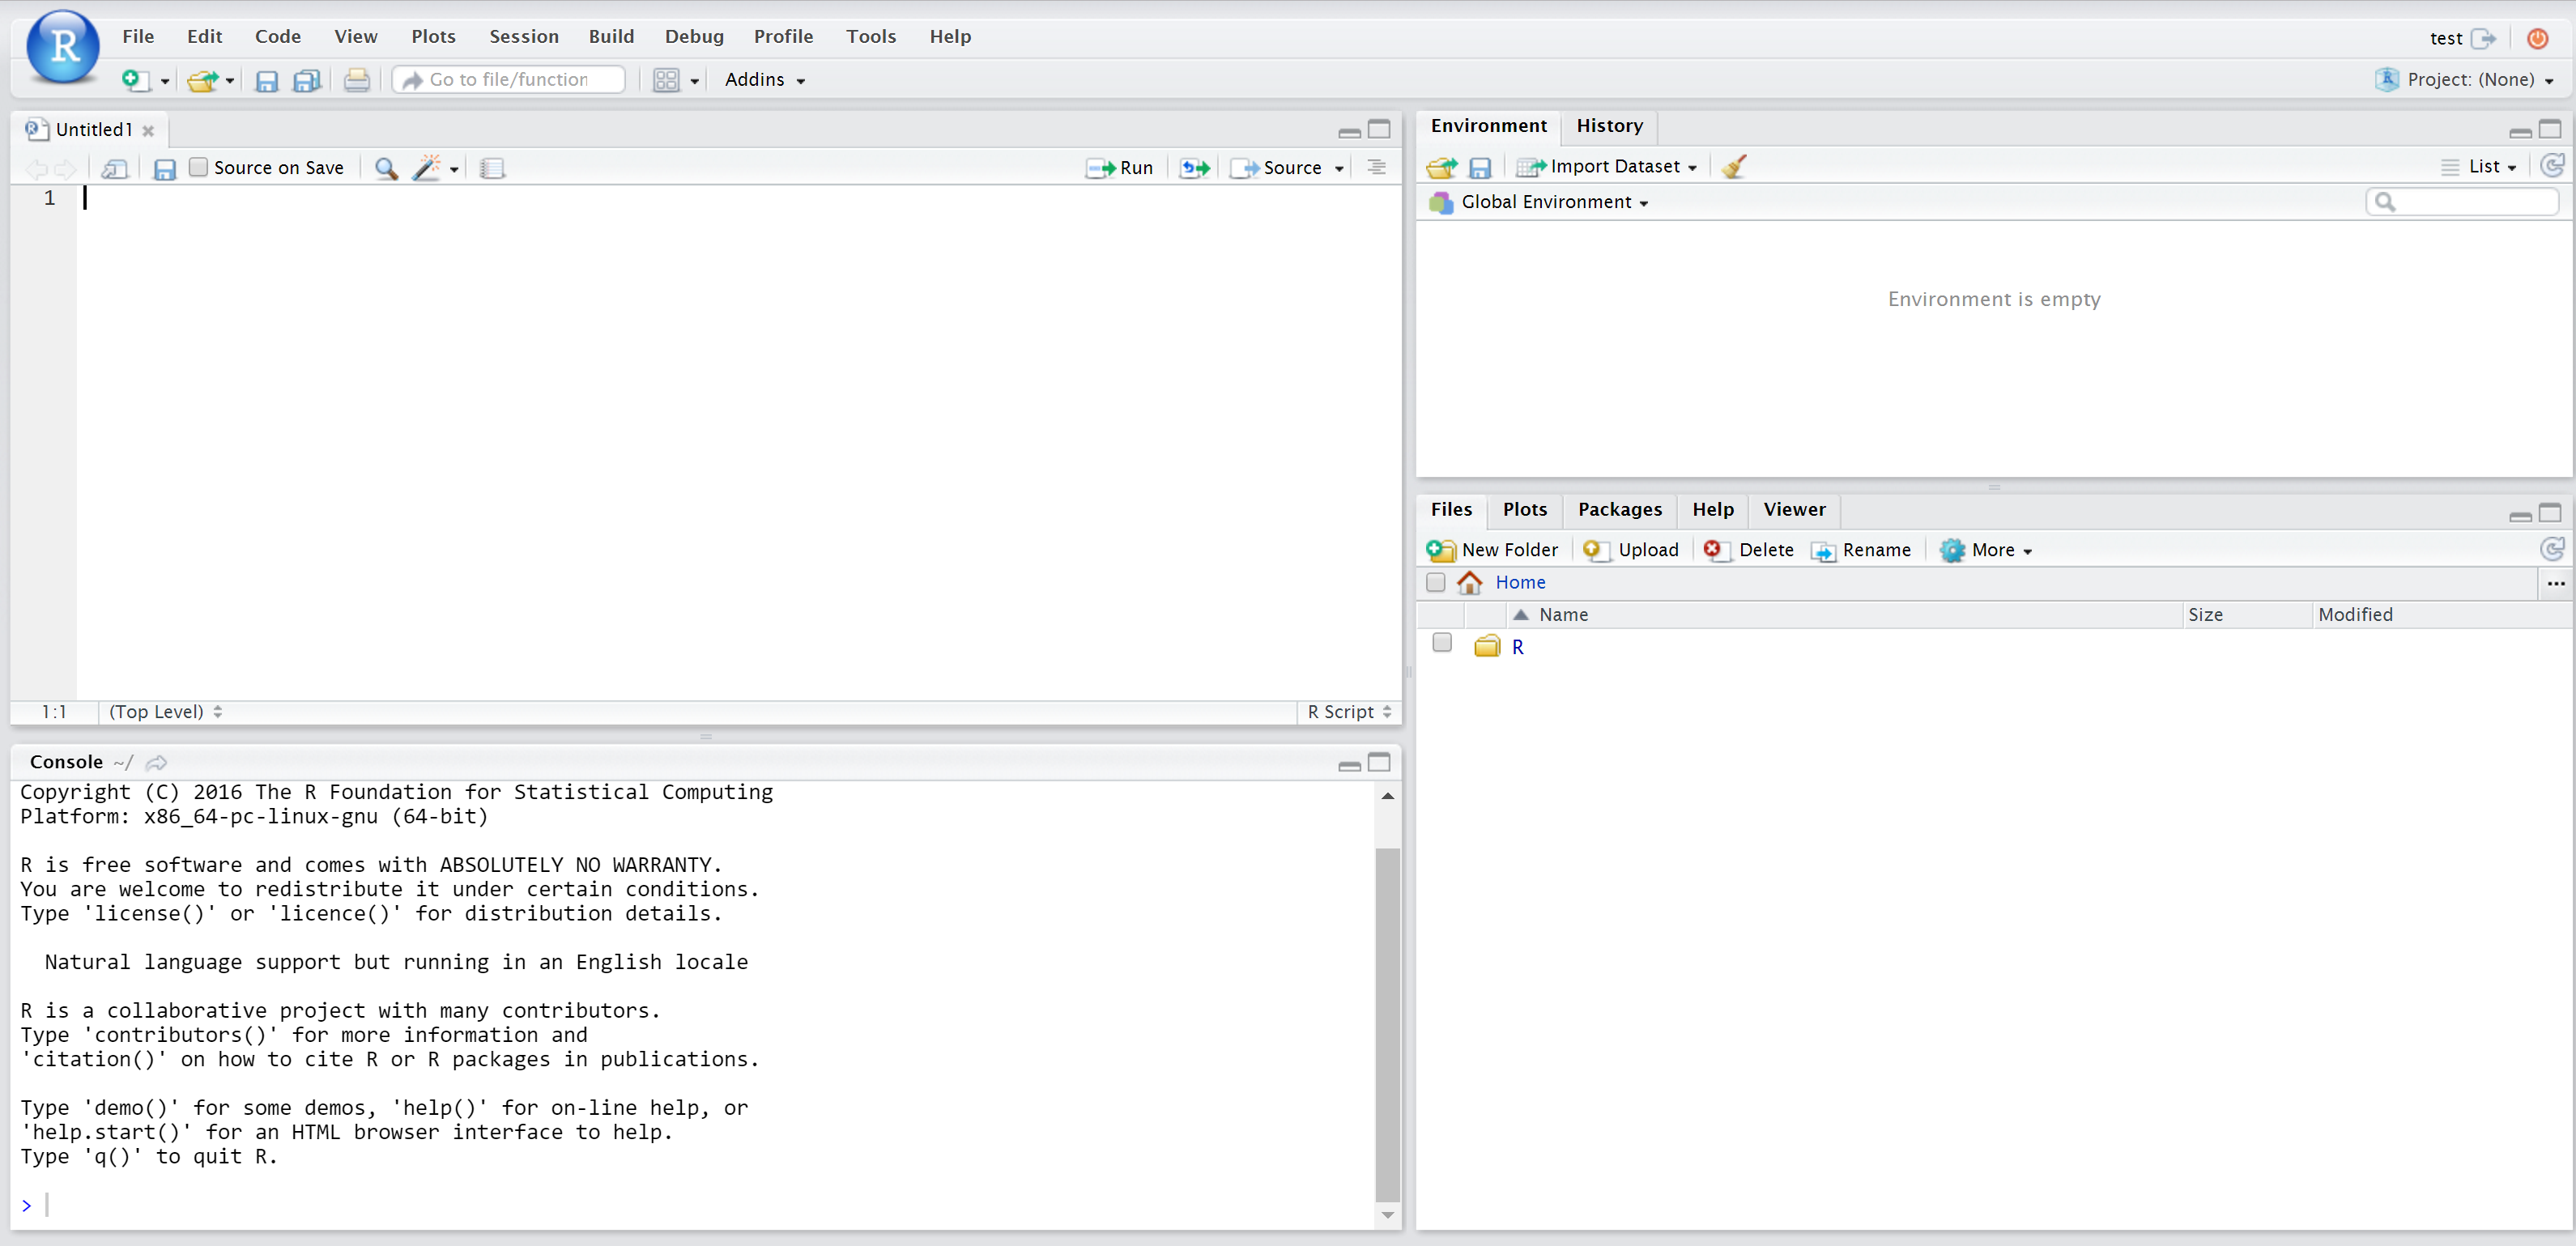
\includegraphics[width=1\textwidth]{console_layout_web}}

The \emph{RStudio} environment is organized by panes, with the default
layout shown above; the script editor and console are on the top and
bottom left, and there are additional panes on the right. The script
editor is used to create and edit files, such as \textsf{R} script
files. Multiple files can be open at once, and will appear as separate
tabs. If the script editor is not visible, open a new file via
\emph{File \textgreater{} New File \textgreater{} R Script} to make the
script editor reappear. When commands are run in the script editor, the
commands and the corresponding output appear in the console.

\emph{RStudio} can be used to create several types of files; the major
two types of files are R Script files (\texttt{.R}) and R Markdown files
(\texttt{.Rmd}). An R Script file contains code that can be executed in
the script editor. Saving code in a script file makes it easy to reuse
or modify code at a later time. An R Markdown file contains both code
and plain text, and can be used to generate a PDF, HTML, or Word
document that contains output (including figures or calculations) along
with the text.

The following section introduces the rest of the \emph{RStudio} layout
and describes the use of the script editor to enter commands. R Markdown
will be introduced in the first lab exercise.

\hypertarget{and-rstudio-tutorial}{%
\section{\texorpdfstring{\textsf{R} and \emph{RStudio}
Tutorial}{ and RStudio Tutorial}}\label{and-rstudio-tutorial}}

\begin{enumerate}
\def\labelenumi{\arabic{enumi}.}
\item
  Open a new R Script file via \emph{File \textgreater{} New File
  \textgreater{} R Script}. While commands can be entered in either the
  script editor or the console, it is recommended to always use the
  script editor; code entered in the editor can be saved, as well as
  easily edited and re-run.
\item
  At its most basic, \textsf{R} can be used as a calculator. Enter
  \texttt{8 + 3} in the script editor and click the \emph{Run} button at
  the top right of the script editor to send the command to the console,
  where the output will appear. Alternatively, with the cursor on the
  line of code, use the keyboard shortcut Ctrl/Cmd + Enter. Try entering
  several lines of arithmetic expressions and running them at once. The
  ``\texttt{\#}'' symbol marks off text as `comments', which are not run
  as code; this is a useful tool for making notes within the code.

\begin{Shaded}
\begin{Highlighting}[]
\CommentTok{#some arithmetic expressions}
\DecValTok{8} \OperatorTok{+}\StringTok{ }\DecValTok{3}
\KeywordTok{log}\NormalTok{(}\DecValTok{2}\NormalTok{)}
\NormalTok{((}\DecValTok{121}\OperatorTok{/}\DecValTok{3}\NormalTok{) }\OperatorTok{*}\StringTok{ }\NormalTok{(}\DecValTok{6}\OperatorTok{^}\DecValTok{3}\NormalTok{))}\OperatorTok{/}\NormalTok{(pi)}
\end{Highlighting}
\end{Shaded}
\item
  The previous calculations only produce output in the console. To save
  a value, assign it a name by using ``\texttt{=}''. Entering the name
  of a value will return the value. For example, run:

\begin{Shaded}
\begin{Highlighting}[]
\CommentTok{#create x and y}
\NormalTok{x =}\StringTok{ }\DecValTok{8} \OperatorTok{+}\StringTok{ }\DecValTok{3}
\NormalTok{y =}\StringTok{ }\KeywordTok{log}\NormalTok{(}\DecValTok{2}\NormalTok{)}

\CommentTok{#calculation}
\NormalTok{x }\OperatorTok{+}\StringTok{ }\NormalTok{y}

\CommentTok{#define and return z}
\NormalTok{z =}\StringTok{ }\NormalTok{x }\OperatorTok{*}\StringTok{ }\NormalTok{y}
\NormalTok{z}
\end{Highlighting}
\end{Shaded}
\item
  Take a look at the Environment tab in the top right
  pane\textemdash the values of \texttt{x}, \texttt{y}, and \texttt{z}
  are displayed. Any created data structures or loaded datasets will
  appear in this tab. All objects can be cleared by selecting the broom
  icon.
\item
  Note that \textsf{R} is case-sensitive; \texttt{x} and \texttt{X} are
  not the same. If you try to run \texttt{X}, an error will be returned
  since no value has been named \texttt{X}. If the same name is used
  again to define a new value, \texttt{R} will overwrite the previous
  information. For example, redefine \texttt{x}:

\begin{Shaded}
\begin{Highlighting}[]
\CommentTok{#a semicolon (;) can be used to separate commands}
\NormalTok{x =}\StringTok{ }\DecValTok{8} \OperatorTok{+}\StringTok{ }\DecValTok{3}\NormalTok{; x}
\NormalTok{x =}\StringTok{ }\DecValTok{21}\NormalTok{; x}
\end{Highlighting}
\end{Shaded}
\item
  Variables can not only contain single values, but also vectors or
  matrices of values. One simple way to create a vector is to use the
  \texttt{c()} command:

\begin{Shaded}
\begin{Highlighting}[]
\CommentTok{#define and return vectors a and b}
\NormalTok{a =}\StringTok{ }\KeywordTok{c}\NormalTok{(}\FloatTok{4.1}\NormalTok{, }\FloatTok{6.7}\NormalTok{, }\FloatTok{8.2}\NormalTok{, }\FloatTok{1.8}\NormalTok{); a}
\NormalTok{b =}\StringTok{ }\DecValTok{2}\OperatorTok{*}\NormalTok{a; b}
\end{Highlighting}
\end{Shaded}
\item
  Use \texttt{mean()} and \texttt{sd()} to find the mean and standard
  deviation of the numbers in \texttt{a}:

\begin{Shaded}
\begin{Highlighting}[]
\CommentTok{#calculate mean and standard deviation}
\KeywordTok{mean}\NormalTok{(a)}
\KeywordTok{sd}\NormalTok{(a)}
\end{Highlighting}
\end{Shaded}
\item
  Plots appear in the Plots tab in the lower right. Plot the values of
  \texttt{a} against the values of \texttt{b}:

\begin{Shaded}
\begin{Highlighting}[]
\CommentTok{#plot a against b}
\KeywordTok{plot}\NormalTok{(a, b)}
\end{Highlighting}
\end{Shaded}
\item
  \textsf{R} has help pages that can sometimes be useful; they typically
  contain a basic description and include syntax information. To look up
  what a certain function does, use \texttt{?}; for example, run
  \texttt{?mean} and the help page for the \texttt{mean} will appear in
  the Help tab on the bottom right.
\item
  The Files tab shows all the files on the local computer; the
  ``\ldots{}'' icon in the upper right corner opens up the directory in
  a separate window, which makes it easier to browse for a particular
  location. Save your script file via \emph{File \textgreater{} Save
  As\ldots{}} in a specific destination, such as the Desktop, then close
  the script file. Use the Files tab in the upper right pane to navigate
  to where the file is saved. Clicking on the script file reopens it in
  the script editor.
\item
  Bonus: the \emph{RStudio} workspace can be customized easily. The
  panels can be rearranged by going to \emph{Tools \textgreater{} Global
  Options \textgreater{} Pane Layout}. Other customization options
  (e.g., font size, themes, etc.) are available under \emph{Global
  Options \textgreater{} Appearance}.
\end{enumerate}

%\showmatmethods





\end{document}

